%%%%%%%%%%%%%%%教案头%%%%%%%%%%%%%%%%%%%%%%%%%%%%%%%
\mode<article>{

\begin{longtable}{|m{20mm}|m{20mm}|m{20mm}|m{20mm}|m{20mm}|m{28mm}|}
\caption*{\huge 教案头}\\
\hline
\endfirsthead
\multicolumn{6}{l}{(续表)}\\
\hline
\endhead
\hline
\multicolumn{6}{l}{\itshape 接下一页表格.......}\\ [2ex]
\endfoot
\hline
\endlastfoot
\centering{授课单元}&\multicolumn{3}{m{60mm}|}{\centering 2.3.1线性元件的微分方程}&\centering{授课日期}&2014年03月13日 \\
\hline
\centering 授课地点 & \multicolumn{3}{m{60mm}|}{B6-204}&\centering 授课学时 & 2 \\
\hline
& \multicolumn{2}{m{40mm}|}{能力目标} & \multicolumn{2}{m{40mm}|}{知识目标}&素质目标 \\
\cline{2-6}
\centering 教学目标&\multicolumn{2}{m{40mm}|}{\begin{enumerate}
\item 能够建立电子网络的一阶和二阶微分方程
\item 能够建立机械系统的一阶和二附微分方程
\end{enumerate} }&\multicolumn{2}{m{40mm}|}{\begin{enumerate}
\item 掌握线性元件微分方程的建立方法
\end{enumerate}} & {\qquad}\\
\hline
\centering 能力训练任务或案例 &\multicolumn{5}{m{108mm}|}{\begin{enumerate}
\item RC网络电路图
\item RLC网络电路图
\item 弹簧-质量-阻尼器机械平移实例
\item 机械转实例
\end{enumerate}}\\
\hline
\centering 教学重点 & \multicolumn{5}{m{108mm}|}{\begin{enumerate}
\item 电子网络的微分方程
\item 机械系统的微分方程
\end{enumerate}}\\
\hline
\centering 教学难点与解决办法 &\multicolumn{5}{m{108mm}|}{\begin{enumerate}
\item 难点:电子网络和机械系统的微分方程
\item 解决方法:补充电子瞬态和机械力方面的知识
\end{enumerate}}\\
\hline
\centering 德育内容 &\multicolumn{5}{m{108mm}|}{无}\\
\hline
 &教材 & \multicolumn{4}{m{88mm}|}{计算机控制原理与应用}\\
\cline{2-6}& 教学资源 &\multicolumn{4}{m{88mm}|}{PPT}\\
\cline{2-6}\centering 使用的教学材料& 主要教学仪器设备和工具等 &\multicolumn{4}{m{88mm}|}{投影机、MATLAB}\\
\cline{2-6}& 主要耗材 &\multicolumn{4}{m{88mm}|}{无}\\
\hline
\centering 教学模式 &\multicolumn{2}{m{40mm}|}{知识讲授}&\centering 教学手段 &\multicolumn{2}{m{48mm}|}{多媒体教学}\\
\hline
\centering 学生成果与过程考核方式 &\multicolumn{5}{m{108mm}|}{无}
\end{longtable}
\clearpage

%%%%%%%%%%%%%%%教学实施过程%%%%%%%%%%%%%%%%%%%%%%%%%%%%
\begin{landscape}

\begin{longtable}{|m{10mm}|m{50mm}|m{50mm}|m{50mm}|m{15mm}|}
\caption*{\huge 教学组织与实施}\\
\hline
\endfirsthead
\multicolumn{5}{l}{\small 接上页}\\
\hline
\multicolumn{1}{|c|}{步骤}&\multicolumn{1}{c|}{教学内容}&\multicolumn{1}{c|}{教师活动}&\multicolumn{1}{c|}{学生活动}&\multicolumn{1}{c|}{时间}\\
\hline
\endhead

\multicolumn{5}{r}{\small 接下页}\\
\endfoot
\hline
\endlastfoot
\multicolumn{1}{|c|}{步骤}&\multicolumn{1}{c|}{教学内容}&\multicolumn{1}{c|}{教师活动}&\multicolumn{1}{c|}{学生活动}&\multicolumn{1}{c|}{时间}\\\hline
引入&\begin{enumerate}
\item 电学线性元件的约束关系
\item 机械系统的约束关系
\end{enumerate} &\begin{enumerate}
\item 补充电学线性元件的约束知识
\item 补充机械系统的约束知识
\end{enumerate} &\begin{enumerate}
\item 学生记录相关知识
\end{enumerate} &10 \\\hline
讲解&\begin{enumerate}
\item 建立RC电子网络微分方程
\end{enumerate}
 &\begin{enumerate}
\item 展示RC电子网络电路图
\item 指导学生建立RC电子网络电路的微分方程
\item 讲解微分方程的建立要点
\end{enumerate} &\begin{enumerate}
\item 学生建立RC电子网络电路的微分方程
\item 学生展示建立的微分方程
\item 学生记录知识要点
\end{enumerate} &15 \\\hline
讲解&\begin{enumerate}
\item 建立RCL电子网络微分方程
\end{enumerate}
&\begin{enumerate}
\item 展示RCL电子网络电路图
\item 指导学生建立微分方程
\item 讲解建立要点
\end{enumerate} &\begin{enumerate}
\item 学生尝试建立微分方程
\item 学生展示建立的微分方程
\item 学生进行记录
\end{enumerate} &20 \\\hline
讲解&\begin{enumerate}
\item 建立机械平移系统的微分方程
\end{enumerate}
 &\begin{enumerate}
\item 展示弹簧-质量-阻尼器机械平移系统实例
\item 指导学生建立微分方程
\item 讲解要点
\end{enumerate} &\begin{enumerate}
\item 学生建立微分方程
\item 学生展示建立的微分方程
\item 学生记录笔记
\end{enumerate} &20 \\\hline
讲解&
\begin{enumerate}
\item 建立机械转动系统的微分方程
\end{enumerate}
 &\begin{enumerate}
\item 展示机械转动系统的实例
\item 指导学生建立微分方程
\item 讲解要点
\end{enumerate} &\begin{enumerate}
\item 学生建立微分方程
\item 学生展示建立的方程
\item 学生记录笔记
\end{enumerate} &20 \\\hline
\centering 本次课总结(评价)&总结本课程内容 &进行知识总结 &学生倾听 &5 \\\hline
\centering 学生学习笔记或工单等检查情况&\multicolumn{4}{m{165mm}|}{\quad}\\\hline
\centering 课后作业&\multicolumn{4}{m{165mm}|}{2-1,2-15,2-17,2-18}\\\hline
\centering 教学体会&\multicolumn{4}{m{165mm}|}{\quad}\\
\end{longtable}

\end{landscape}
\clearpage
%%%%%%%%%%%%%%%%%%%%板书设计%%%%%%%%%%%%%%%%%%%%%%%%%%
\lecture{物理系统的数学模型}{wulimoxing}
\begin{center}
{\huge 板书设计}
\end{center}
}
\mode<presentation>{ \section{线性元件的微分方程}
 \subsection{电子网络}}
\begin{frame}[containsverbatim]{电子网络}
\begin{circuitikz}[american]
\draw(0,0)to[generic,l^=$R$,o-*](3,0)to[C,l=$C$](3,-2)to[short,*-o](0,-2)to[open,o-,l=$v_{1}(t)$](0,0)(3,0)to[short,-o](5,0)to[open,-o,l=$v_{o}(t)$](5,-2)to[short](3,-2);
\end{circuitikz}
 \end{frame}
 \begin{frame}{电气元件的基本关系}
\uncover<+->{ 电阻:
 \[R=\frac{v_{r}(t)}{i(t)}\]}
\uncover<+->{ 电容:
 \[v_{c}(t)=\frac{1}{C}\int{i(t)}dt\]}
 \uncover<+->{电感:
 \[v_{L}(t)=\frac{di(t)}{dt}\]}
 \end{frame}
 \begin{frame}
\uncover<+->{ \[v_{1}(t)=Ri(t)+v_{o}(t)\]}
 \uncover<+->{由:
 \[i(t)=C\frac{dv_{0}(t)}{dt}\]}
\uncover<+->{得:
\[v_{1}(t)=RC\frac{dv_{o}(t)}{dt}+v_{o}(t)\]}
\uncover<+->{整理得:
\[\frac{dv_{o}(t)}{dt}+\frac{1}{RC}v_{o}=\frac{1}{RC}v_{1}(t)\]}
 \end{frame}
 \begin{frame}
\uncover<+->{ \begin{circuitikz}[american]
 \draw(0,0)to[generic,l^=$R$,o-](2,0)to[L,l^=$L$](4,0)to[C,l=$C$,*-*](4,-2)to[short,-o](0,-2)to[open,l=$v_{1}(t)$](0,0)(4,0)to[short,-o](6,0)to[open,l=$v_{o}(t)$,-o](6,-2)to[short](4,-2);
 \end{circuitikz}}
 \uncover<+->{\[v_{1}(t)=v_{R}(t)+v_{L}(t)+v_{o}(t)\]}
\uncover<+->{\[v_{1}(t)=RC\frac{v_{o}(t)}{dt}+LC\frac{d^{2}v_{o}(t)}{dt^{2}}+v_{o}(t)\]}
 \end{frame}
 \begin{frame}
 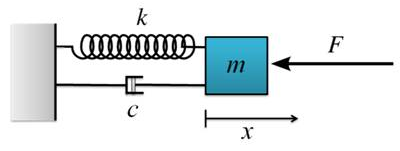
\includegraphics[scale=0.8]{tanhuangzuni.png}
 \end{frame}
 \begin{frame}{机械系统}
 平移系统:
 \uncover<+->{\[ma=\Sigma F\]}
 \uncover<+->{\[a=\frac{d^{2}y(t)}{d^{2}t}\]}
\uncover<+->{ \[F_s =-ky(t)\]}
\uncover<+->{ \[f_b=-c\frac{dy(t)}{dt)}\]}
 \end{frame}
 \begin{frame}{机械系统}
 \uncover<+->{转动系统:
 \[J\alpha =\Sigma T\]}
\uncover<+->{\[
 \alpha =\frac{d\omega (t)}{dt}=\frac{d^{2}\theta (t)}{dt^2}\]}
\uncover<+->{ \[F_b=-c\omega(t)=-c\frac{d\theta(t)}{dt}\]}
 \end{frame}
 
\endinput